\documentclass[a4paper,12pt]{article}
\usepackage[spanish]{babel} 
\usepackage{amsmath} 
\usepackage[colorlinks=true]{hyperref}
\usepackage{enumitem} 
\usepackage{graphicx}   
\usepackage[a4paper,top=3cm,bottom=3cm,left=3cm,right=3cm,marginparwidth=1.75cm]{geometry} 
\usepackage[]{subfigure}
\usepackage[]{multicol}

\graphicspath{ {./imag/Lab-Termo/Git/Documentos}} 
\title{Jaula de Faraday} 
\author{Noemi de la Peña, Benjamín Opazo, Martina Contreras \\ \\
 \textit{ Departamento de Física, Universidad de Concepción, Concepción, Chile. }}
  \date{} 

  



   %==================================================================================
\begin{document}
\maketitle 



%=============Resumen.
En este presente documento se expondra datos y concluciones 
obtenidas a traves de 3 diferentes experimentos.Relacionados con el campo electrico,
conductores y las ondas electro magneticas.



%========Introducción
\section*{Introdución}
    A medida que el saber del humano crecee, tambien lo hace las preguntas.
    ¿Porque al frotar un globo sobre mi cabeza los pelos se levantan? o 
    ¿Por qué cae un rayo?
    Los antiguos griegos dieron incapie a el estudio de la ciencia que 
    lograria dar respuesta a las anteriores interrogantes, la electroestatica.

    La electrostática es una rama de la Física que estudia los efectos producidos 
    en los cuerpos como consecuencia de sus cargas eléctricas, o lo que es lo mismo, 
    el comportamiento de las cargas eléctricas en situación de equilibrio.






%========Objetivos
%\section{Objetivos}
%\begin{itemize}
   
%\end{itemize}


%=========Marco Teórico
%\section{Marco Teórico}




%=========Materiales
\section*{Materiales}
\begin{multicols}{2}
\begin{itemize}
    \item celular
    \item papel de aluminio
    \item jabón
    \item agua
    \item globo
    \item bombilla
    \item bolsa ziploc
    \item audífonos
    \item colador de metal 
\end{itemize}
\end{multicols}


%%%%%%%%%%%%%%%%%%%%%%%%Procedimiento
\section*{Experimento 1}
\textit{Materiales: Papel de aluminio, celular.}
\begin{itemize}
    \item Primero, ponemos el celular sobre el papel de aluminio.
    \item Segundo, desde otro móvil, llamamos al celular del esperimento para comprobar que funciona correctamente.
    \item Luego envolvemos el celular con el papel de aluminio.
    \item Finalmente volvemos a llamar, para notar el efecto que tiene el papel de alumio sobre el celular.
\end{itemize}
%Imagenes%
\begin{figure}[h]
    \begin{subfigure}
        \raggedright
        \includegraphics[width=4cm, height=5cm]{imag/Exp1_00.jpg}
        \end{subfigure}
    \begin{subfigure}
        \centering
        \includegraphics[width=4cm, height=5cm]{imag/Exp1_01.jpg}
    \end{subfigure}
    \begin{subfigure}
        \raggedleft
        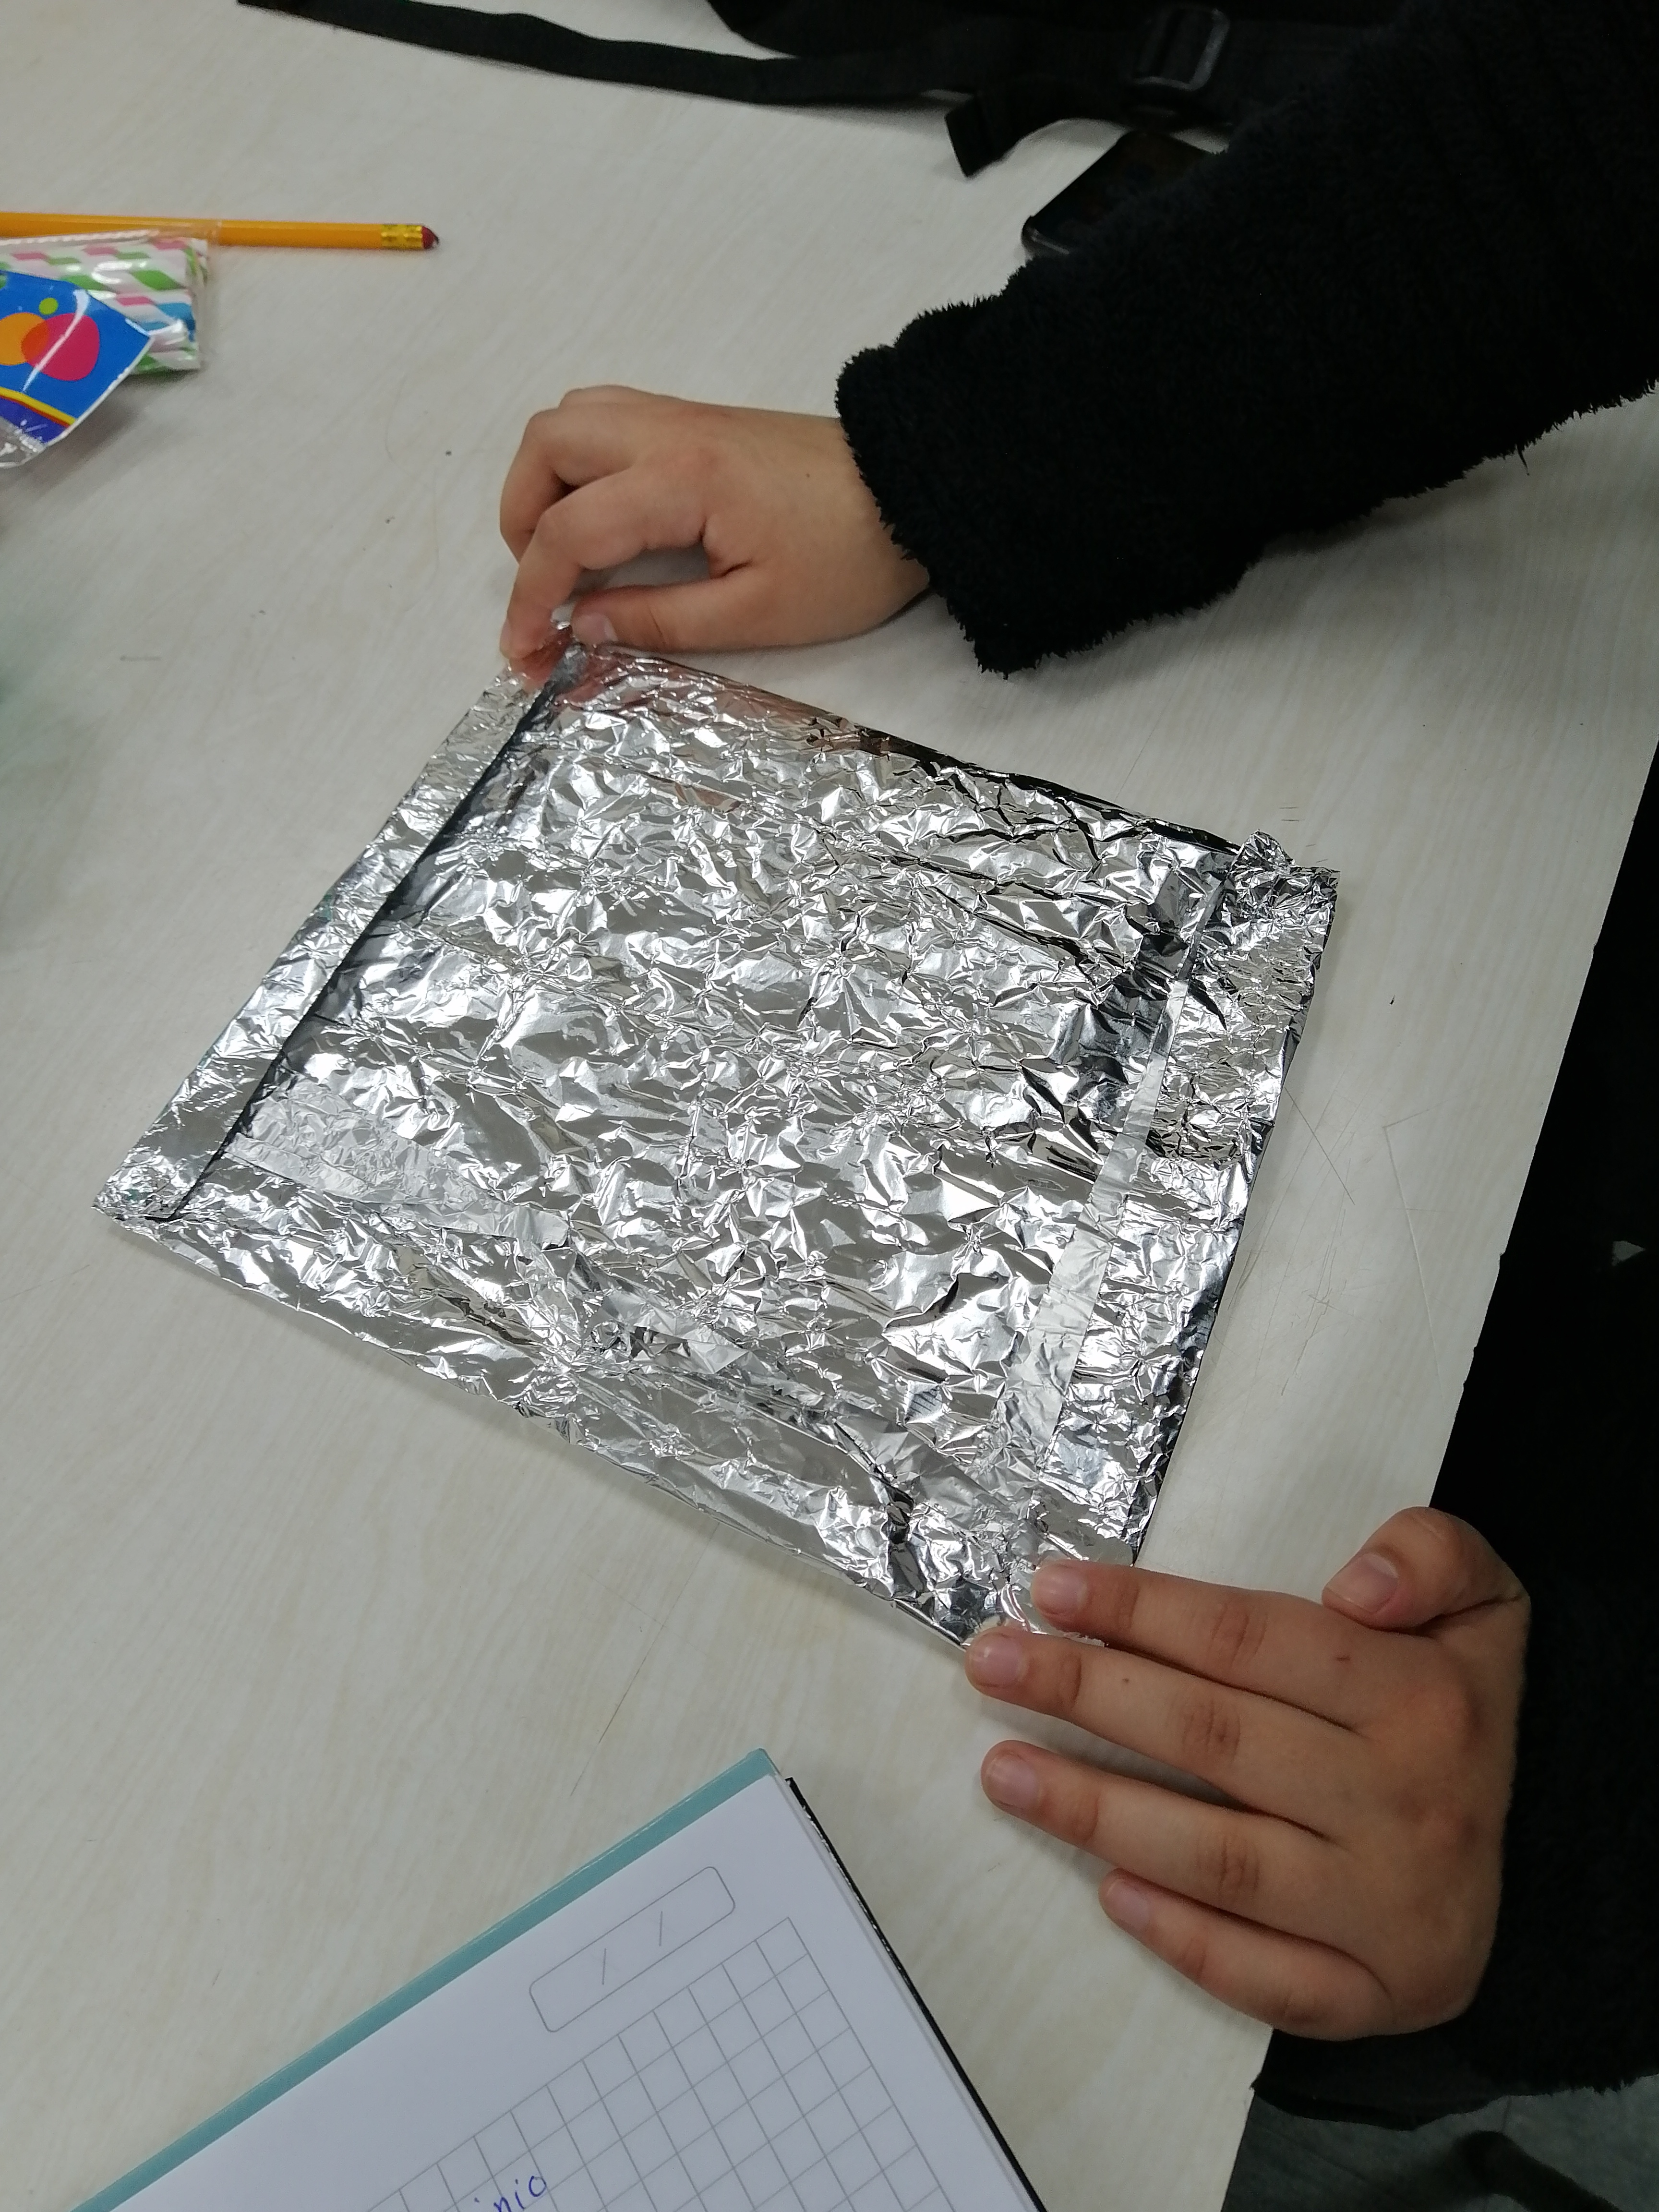
\includegraphics[width=4cm, height=5cm]{imag/Exp1_02.jpg}
    \end{subfigure}
\end{figure}
%%%%%%%%%%%%%%%%%%%%%%%%%%%%%%%%%%%%%%%%%%%%%%%%%%%%%%%%%%

\section*{Experimento 2}
\textit{Materiales: Jabón, agua, bombilla, globo, bolsa ziploc.}
\begin{itemize}
    \item Primero mezclamos el agua con el jabón.
    \item Segundo, sobre la bolsa ziploc, desparramamos un poco de la mezcla hecha anteriormente.
    \item Luego, con una bombilla hacemos una burbuja grande y acercamos el globo, ya inflado, para notar el efecto que tiene sobre la burbuja.
    \item Despues, volvemos hacer otra burbuja,pero en el interior de la burbuja inicial y repetimos el procedimiento hecho con el globo.
\end{itemize}

%Imagenes%
\begin{figure}[h]
    \begin{subfigure}
        \raggedright
        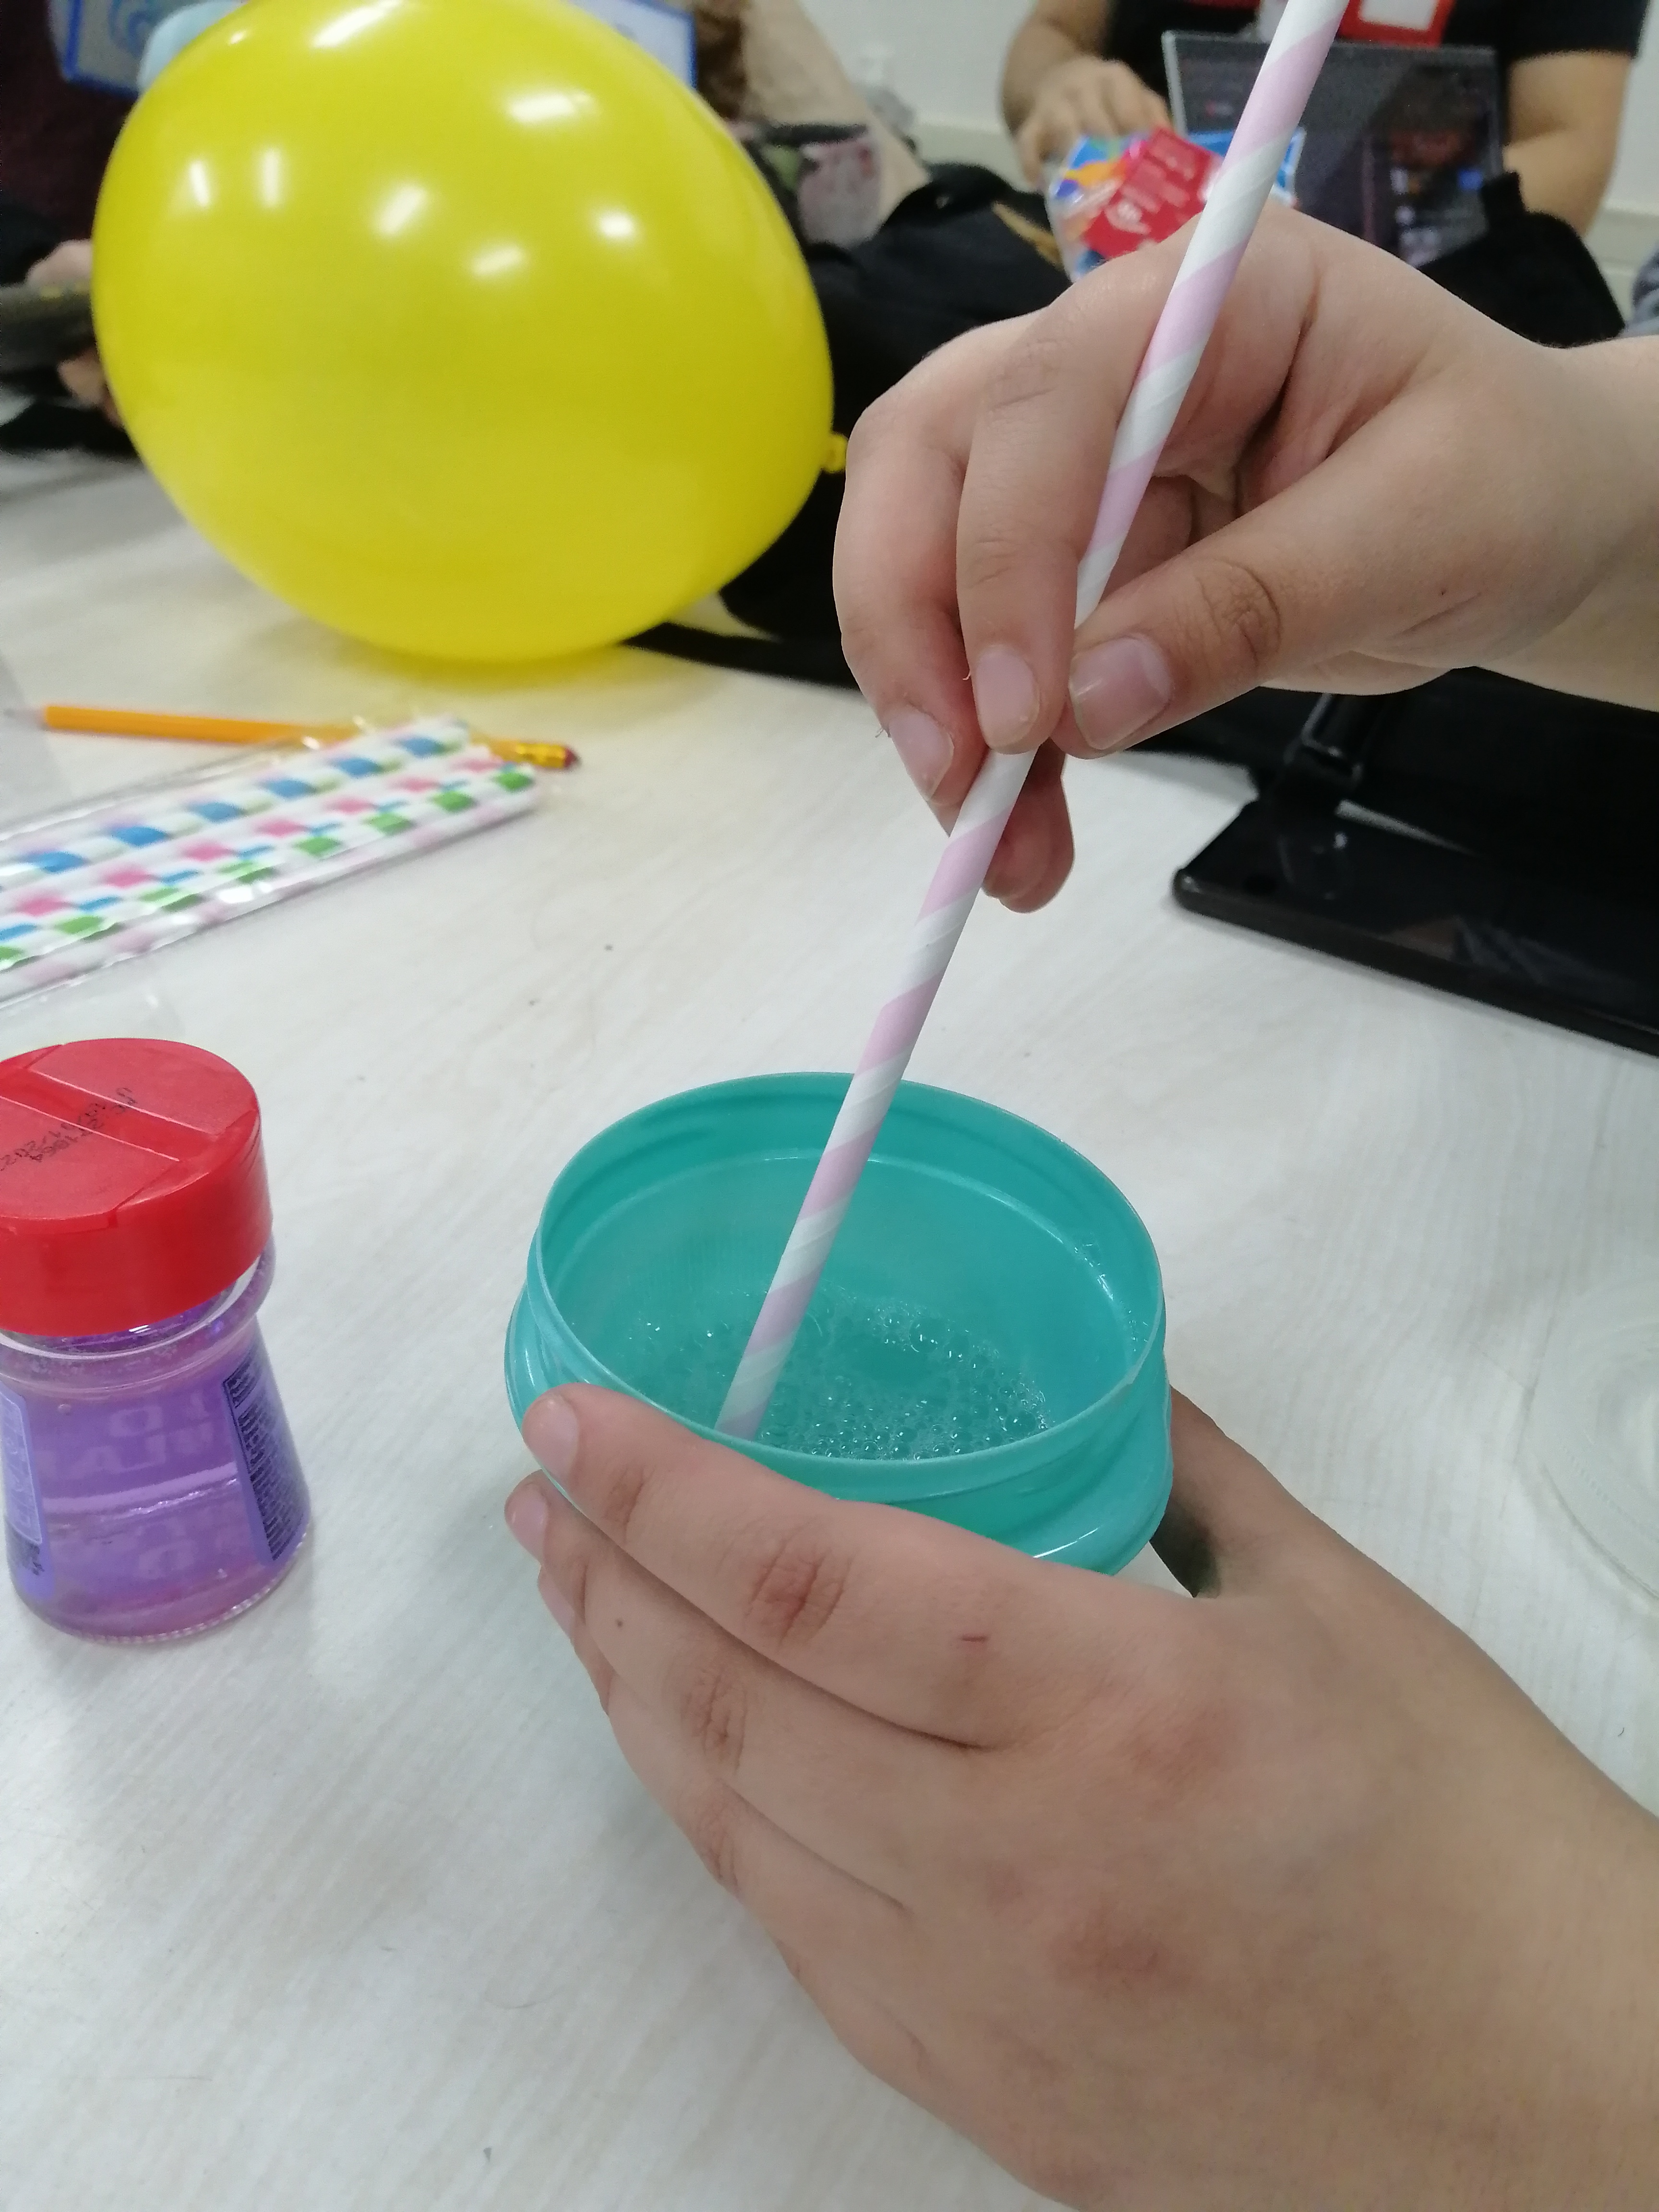
\includegraphics[width=4cm, height=5cm]{imag/Exp2_00.jpg}
    \end{subfigure}
    \begin{subfigure}
        \centering
        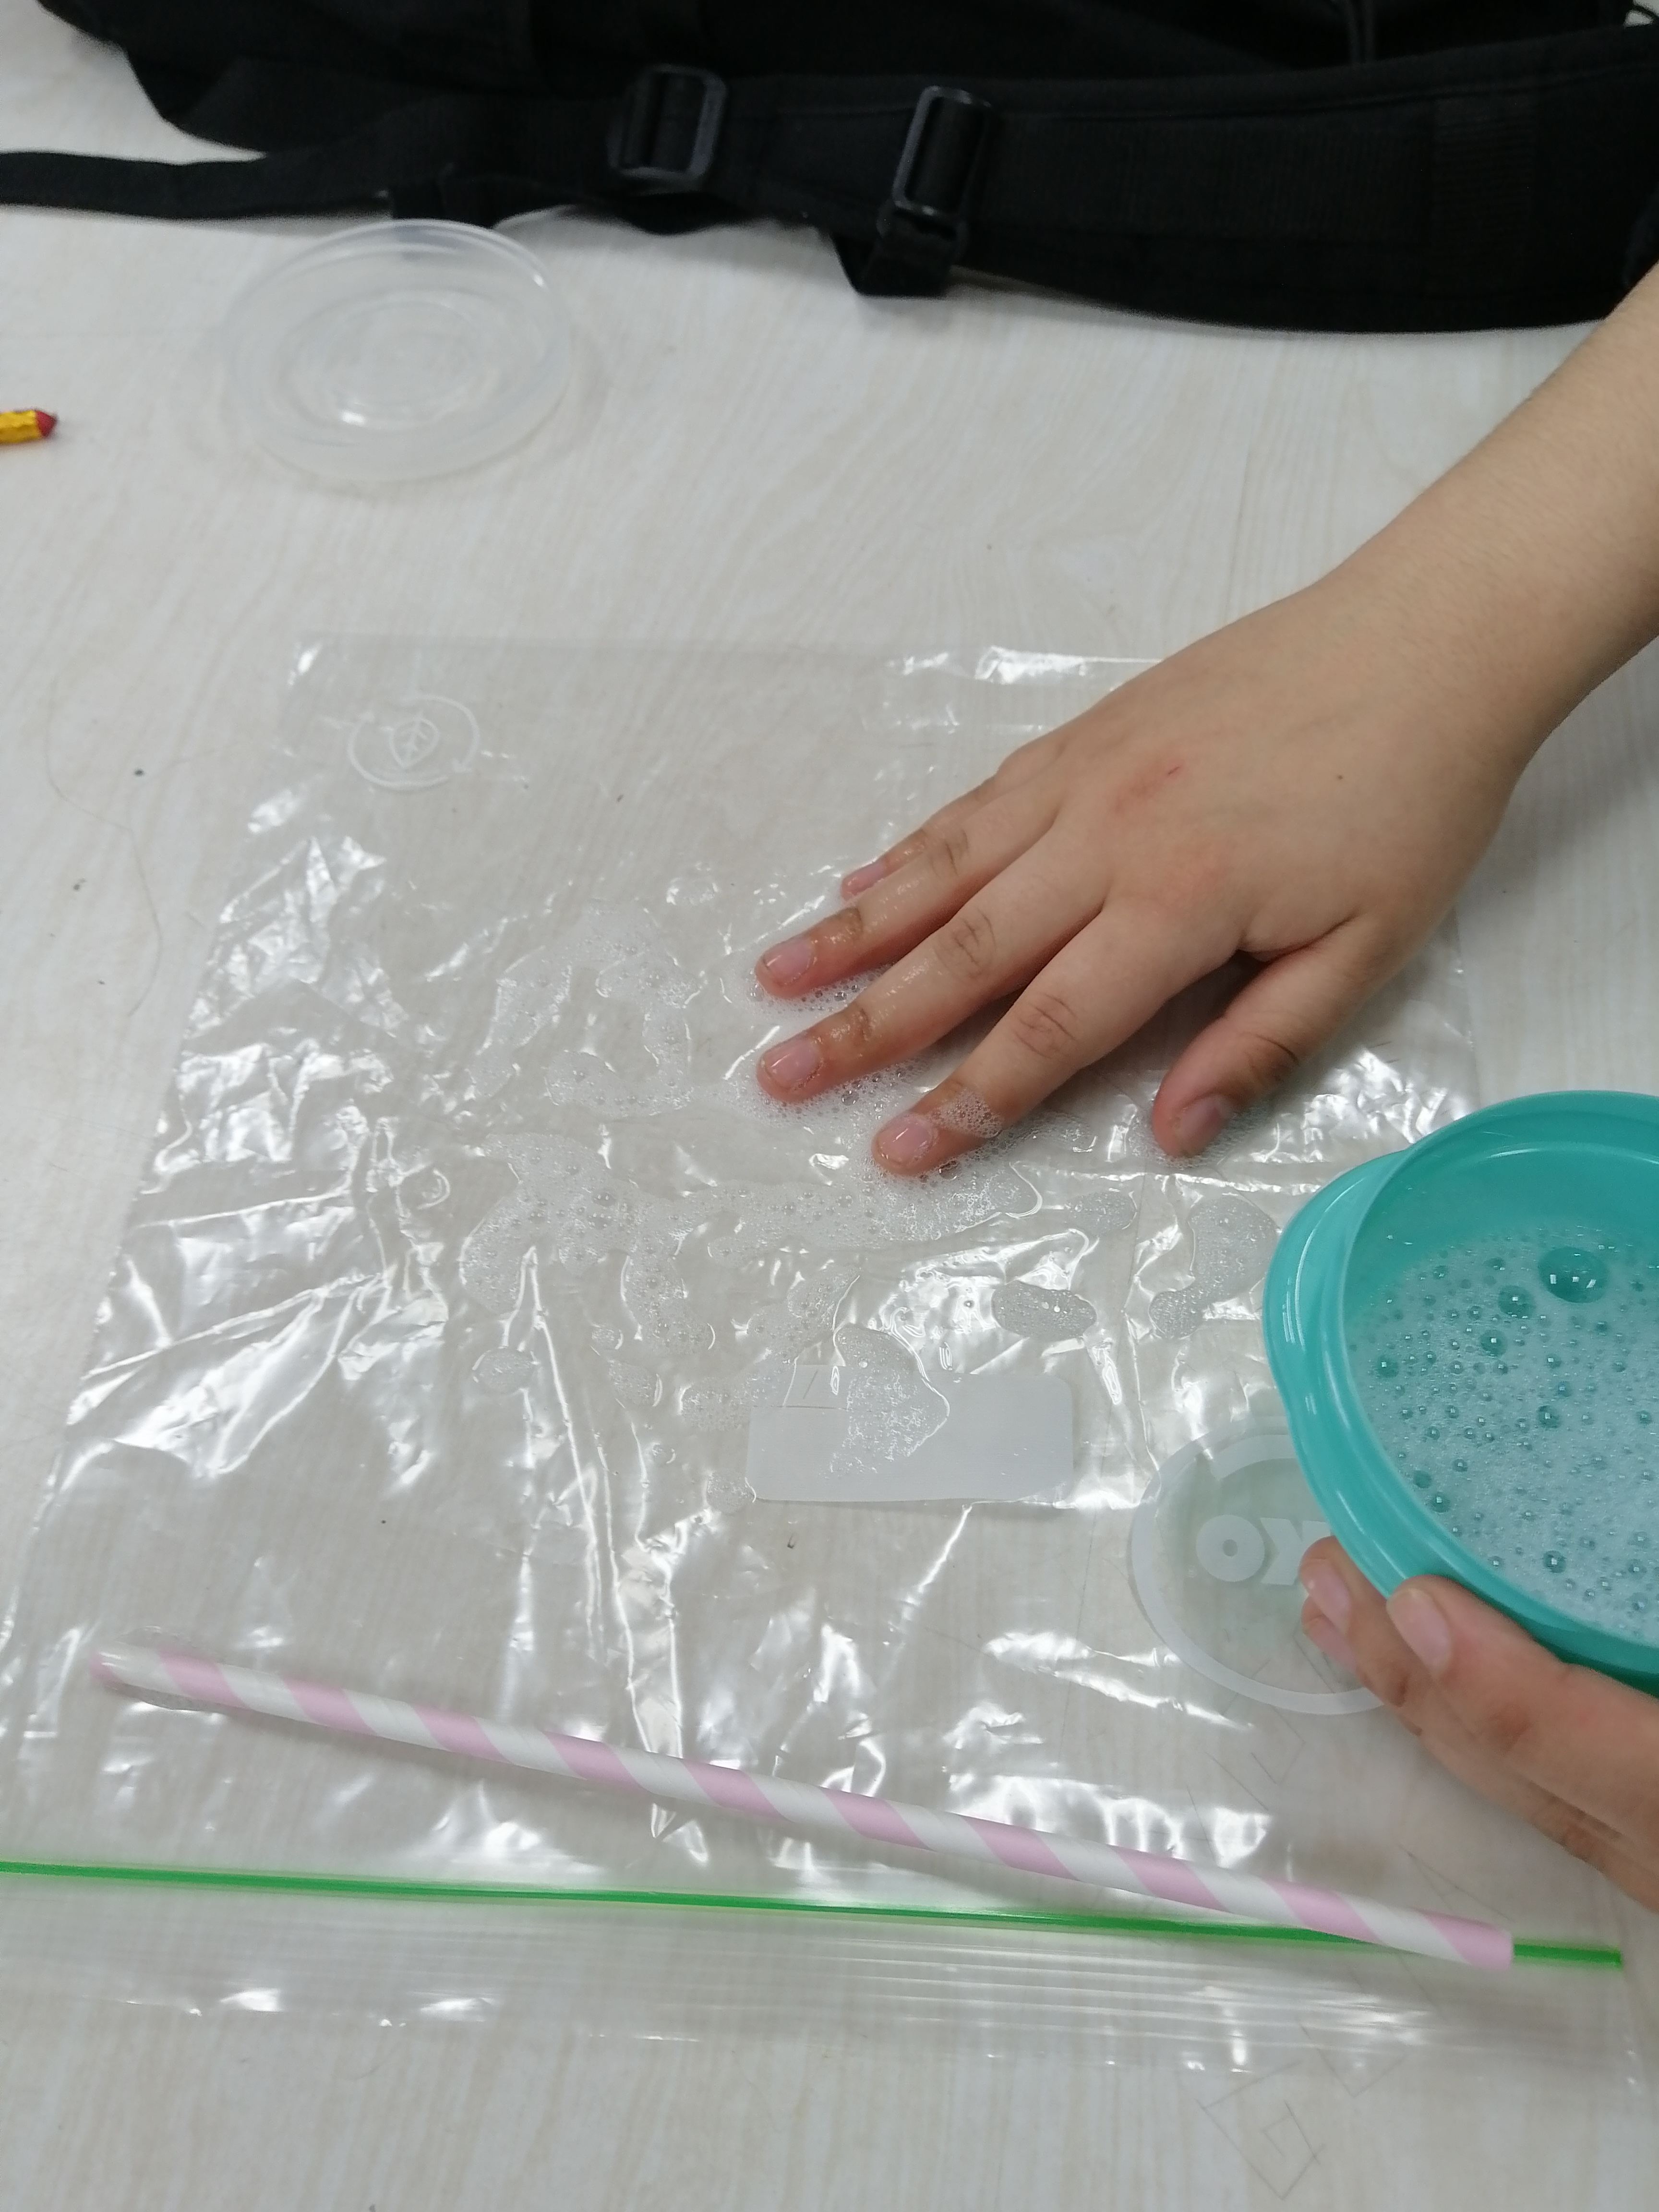
\includegraphics[width=4cm, height=5cm]{imag/Exp2_01.jpg}
    \end{subfigure}
    \begin{subfigure}
        \raggedleft
        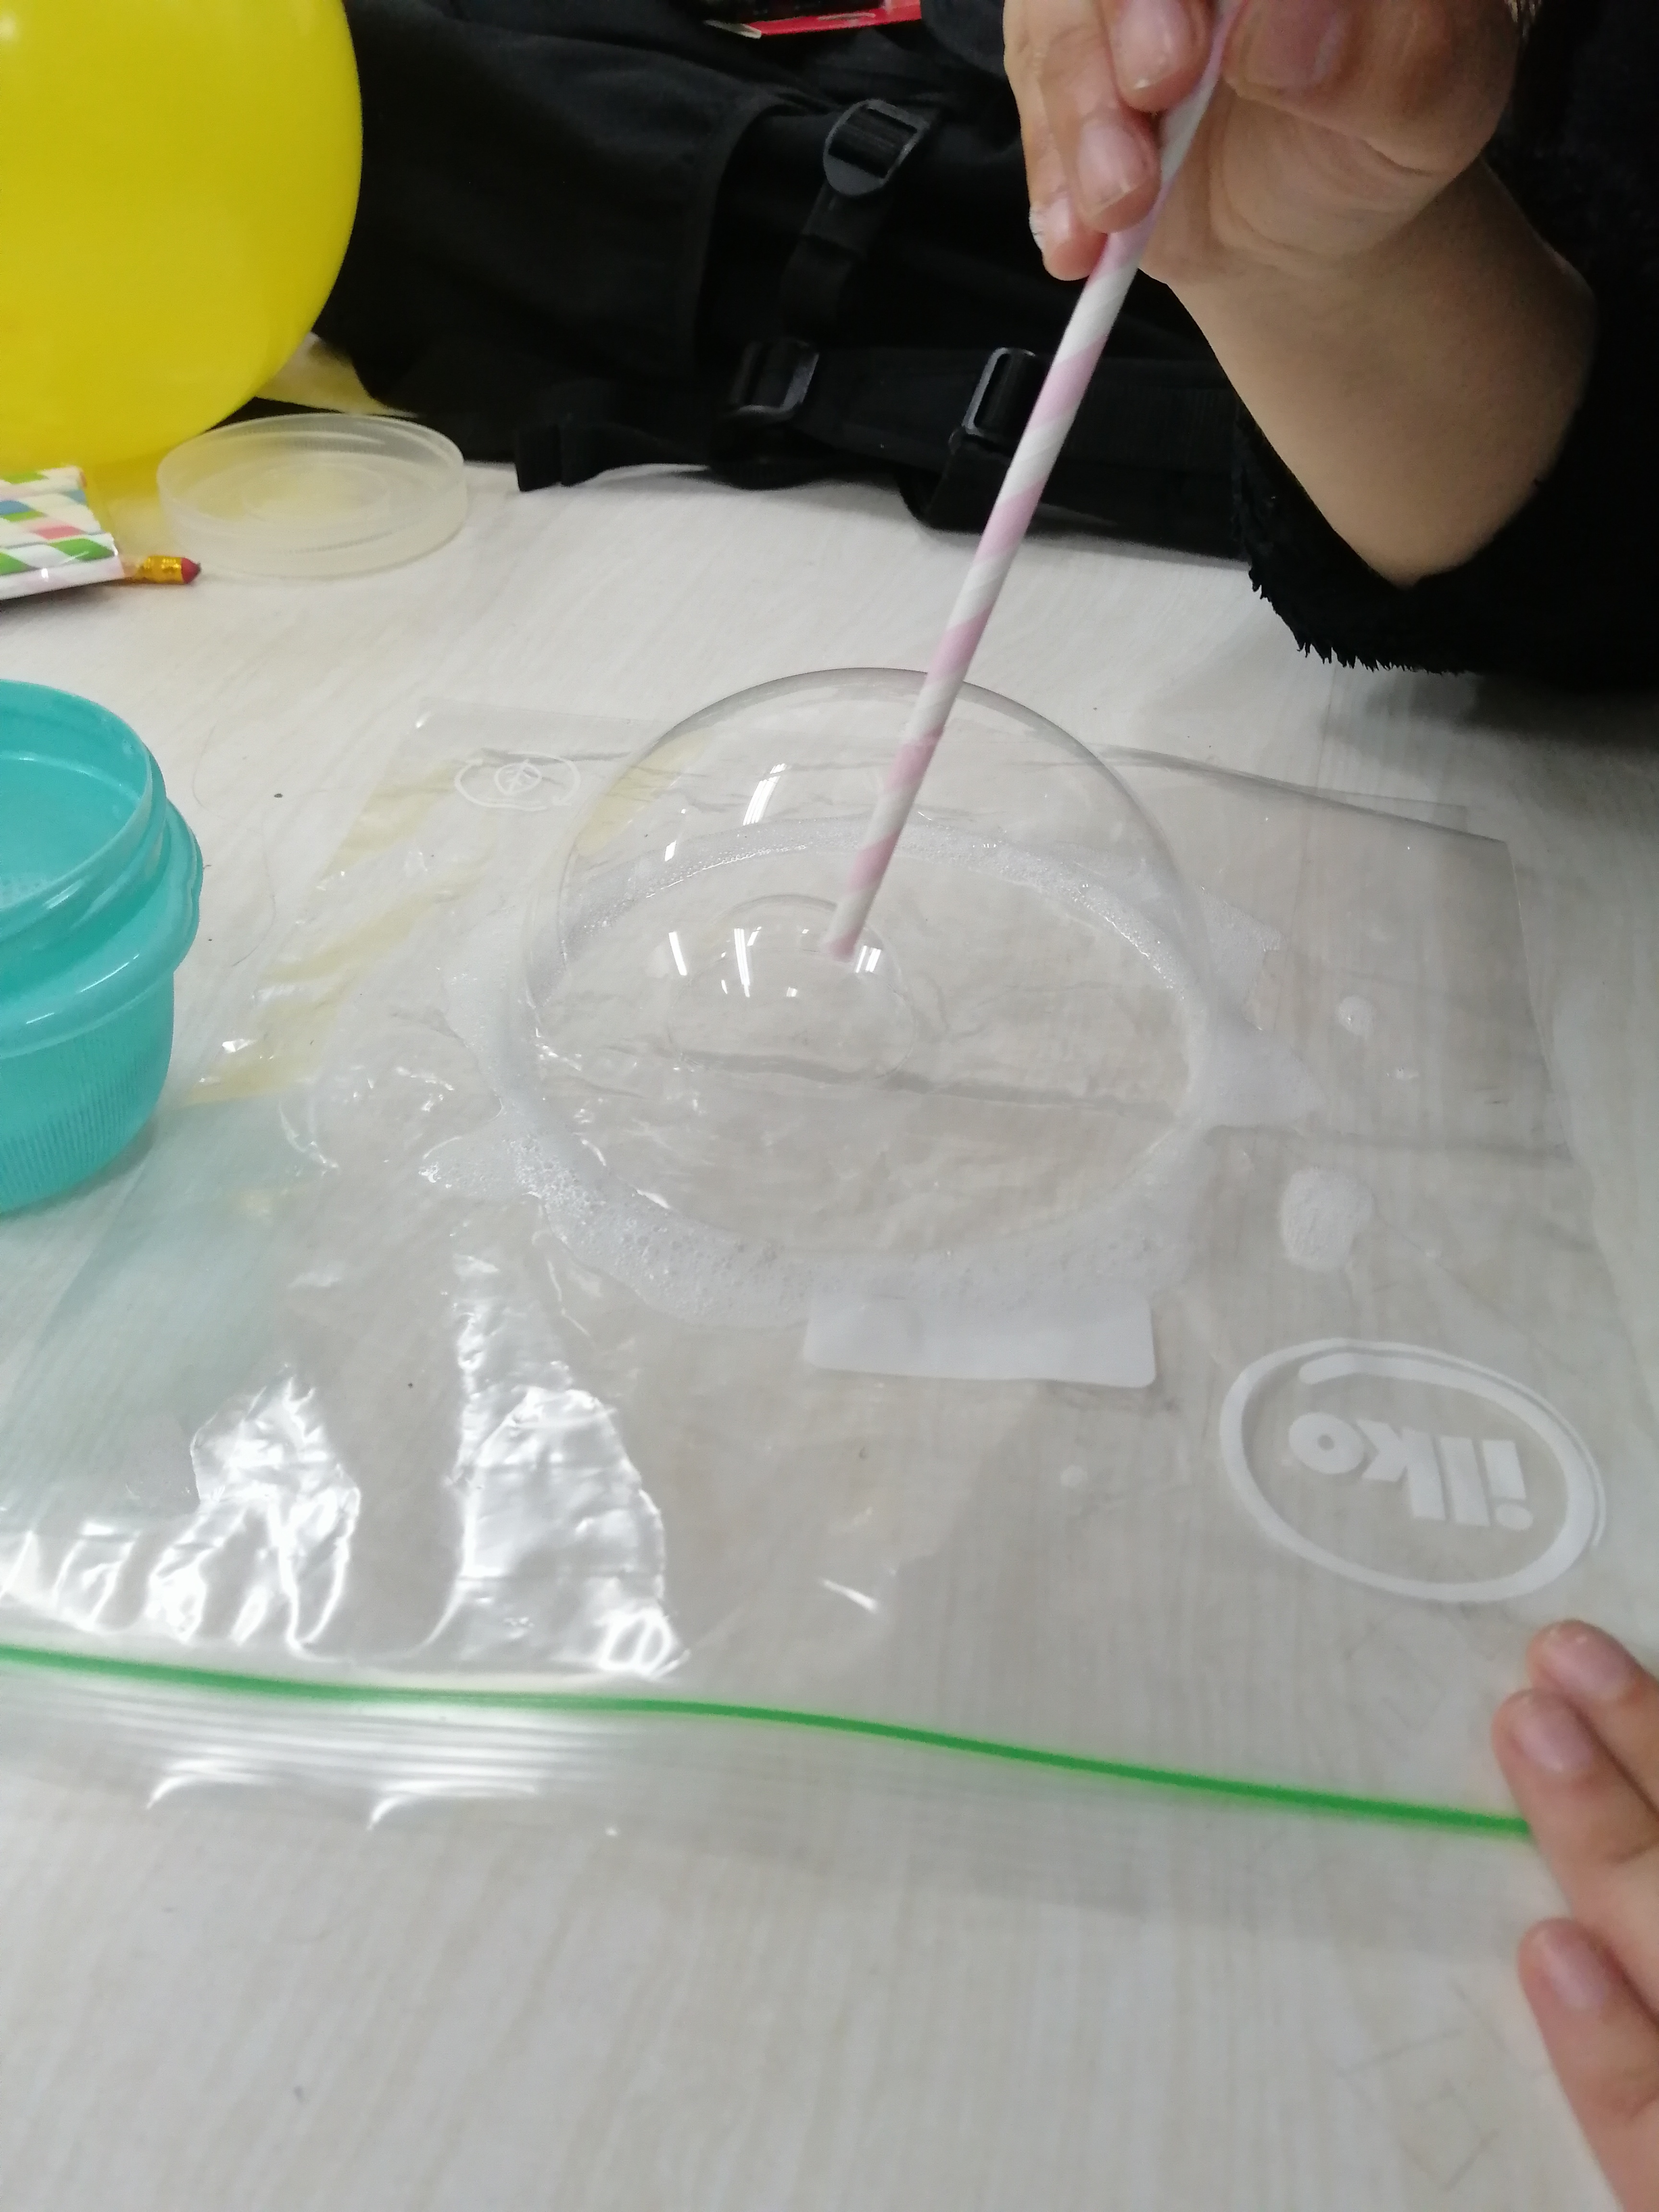
\includegraphics[width=4cm, height=5cm]{imag/Exp2_02.jpg}
    \end{subfigure}
\end{figure}


\begin{figure}[h!]
    \begin{subfigure}
        \raggedright
        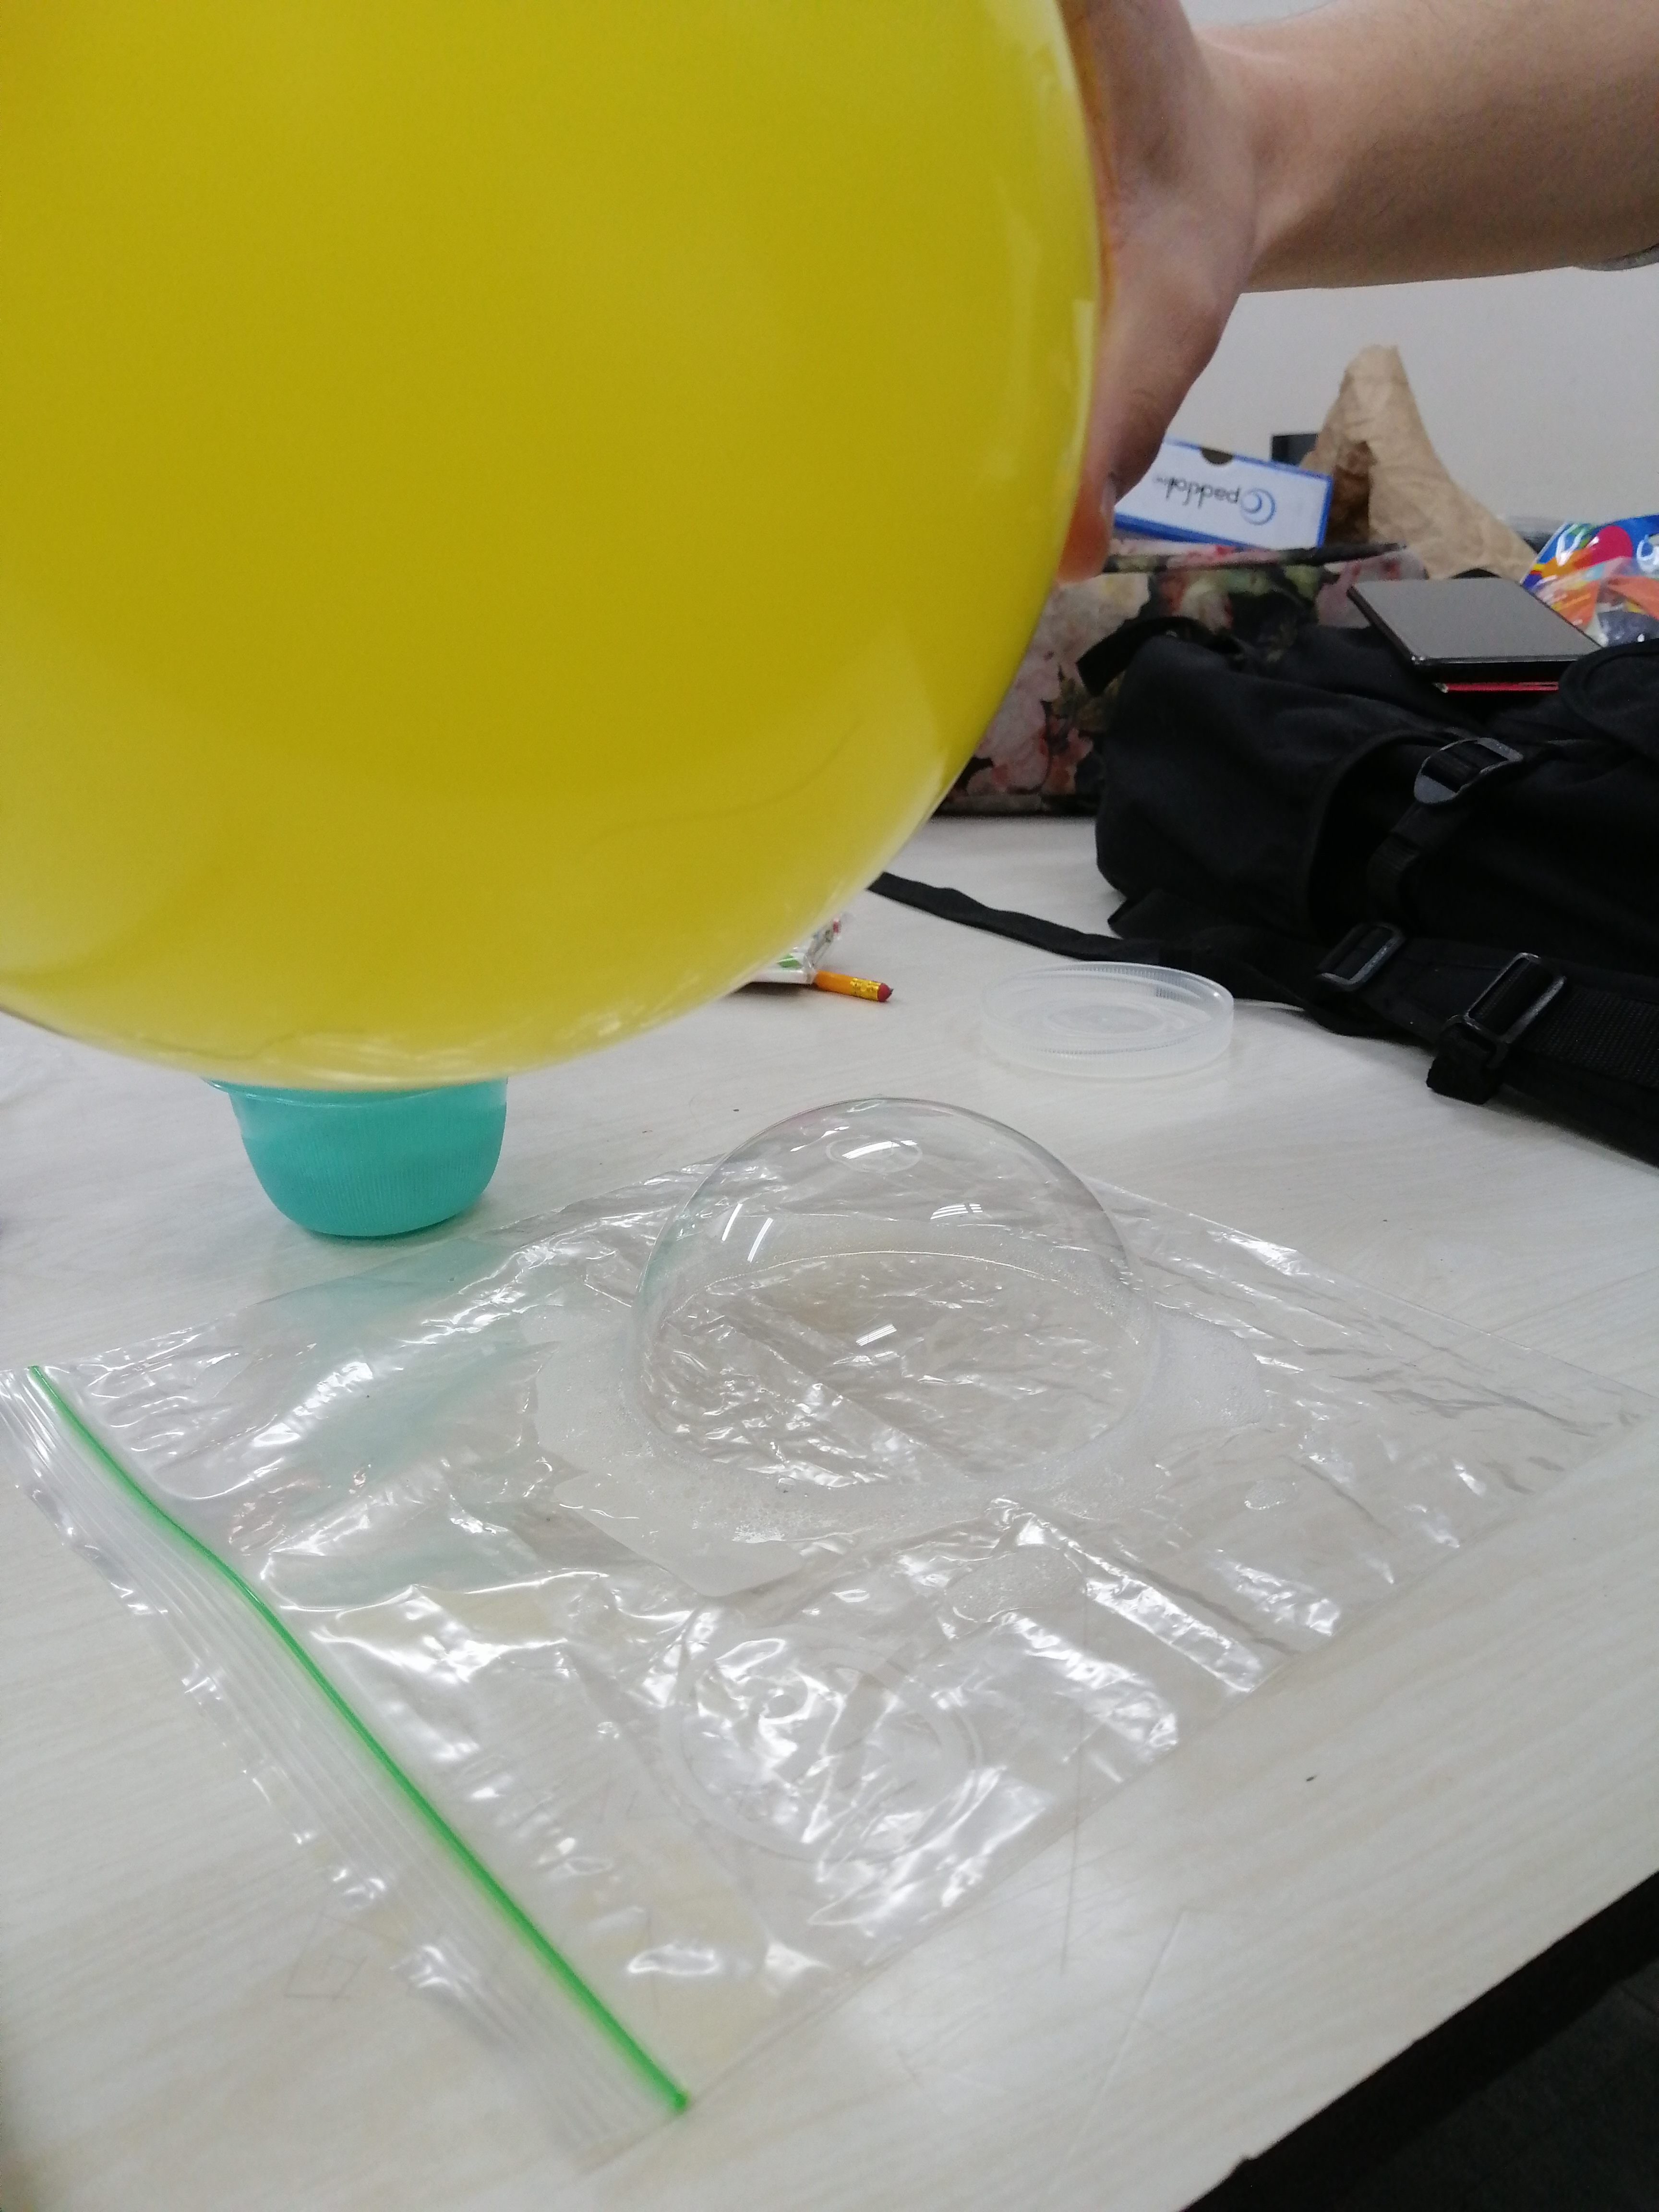
\includegraphics[width=4cm, height=5cm]{imag/Exp2_03.jpg}
    \end{subfigure}
    \begin{subfigure}
        \centering
        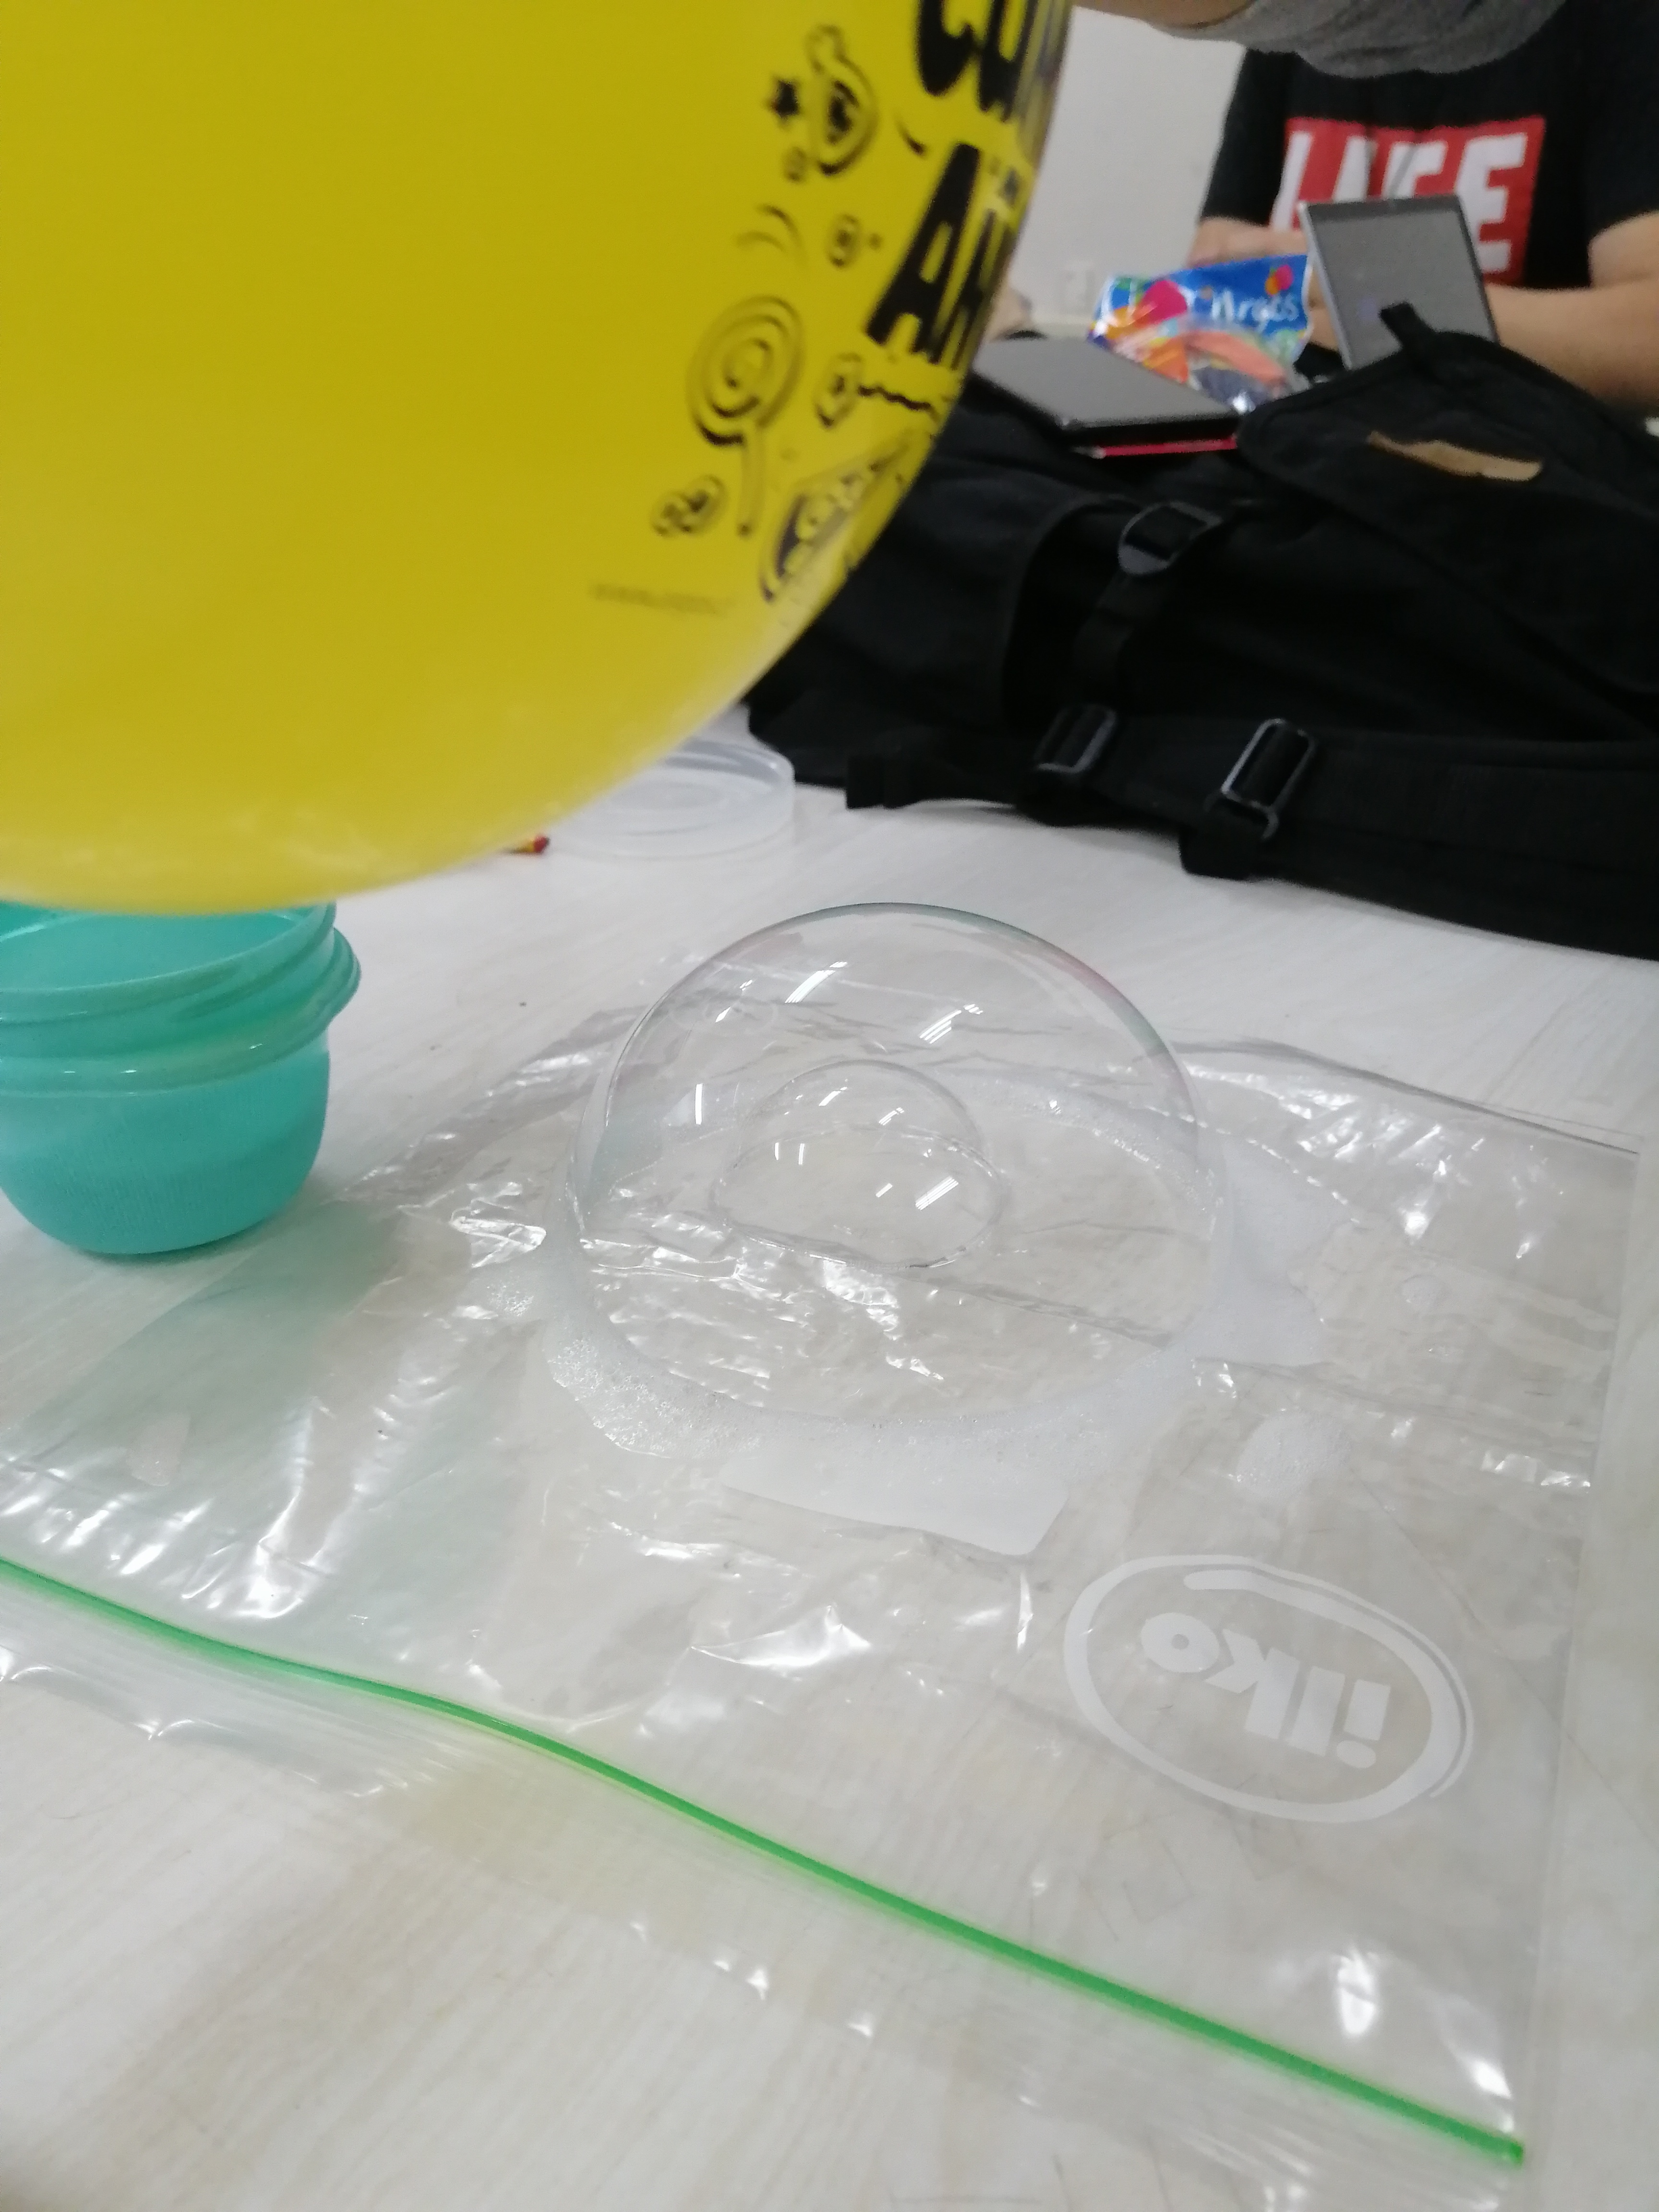
\includegraphics[width=4cm, height=5cm]{imag/Exp2_04.jpg}
    \end{subfigure}
\end{figure}
%%%%%%%%%%%%%%%%%%%%%%%%%%%%%%%%%%%%%%%%%%%%%%%%%%%%%%%%%%%%%%%%%%%%%%%
\newpage
\section*{Experimento 3}
\textit{Materiales: Colador de metal, celular, audífonos, papel de aluminio.}
    \begin{itemize}
        \item Encendermos la radio del celular.
        \item Luego, ponemos el móvil sobre el papel de aluminio.
        \item Finalmente, con el colador de metal, encerramos el área en donde se encuentra el celular.
    \end{itemize}

%imagenes%
\begin{figure}[h!]
    \begin{subfigure}
        \raggedright
        \includegraphics[width=4cm, height=5cm]{imag/Exp3_00.jpg}
    \end{subfigure}
    \begin{subfigure}
        \centering
        \includegraphics[width=4cm, height=5cm]{imag/Exp3_01.jpg}
    \end{subfigure}
\end{figure}













































\end{document}